\section{Discovery and Integration Framework}
\label{sec:framework}

The Semtools project has focused development efforts on three main
components: a Java library for accessing and manipulating OBOE
ontology extensions and semantic annotations, an annotation plugin for
the Morpho metadata editor, and query extensions for the Metacat data
catalog. Below we briefly describe these components and give a brief
overview of the OBOE model (for more in-depth presentation of OBOE see
\cite{madin07:_ontol_for_descr_and_synth,bowers08}) and the semantic
annotation approach used in Semtools.


\mypara{The OBOE Observational Model.}  \figref{fig:oboe} shows the
main modeling constructs of
OBOE\footnote{\url{http://ecoinformatics.org/oboe/oboe.1.0/oboe-core.owl}}. An
{\em observation} is made of an {\em entity} (e.g., biological
organisms, geographic locations, environmental features) and serves to
group a set of measurements together to form a single
``\emph{observation event}''. A \emph{measurement} assigns a value to
a {\em characteristic} of the observed entity (e.g., the weight of a
plant), and can also include \emph{standards} (e.g., units) and
collection \emph{protocols}. An observation can occur within the
surrounding \emph{context} of other observations (e.g., as part of a
temporal or spatial context), and context may include a named
relationship (e.g., ``partOf'', ``within'') that existed during the
observation event. A key feature of OBOE is that it allows properties
(characteristics and relationships) of entities to be asserted without
being interpreted as \emph{inherently} (i.e., {always}) true of the
entity.  Depending on the context in which the entity was observed or
how the measurements were performed, an entity's properties may take
on different values.  OBOE allows RDF-style assertions about entities
to be contextualized, and thus different values can be assigned for
the same entity under distinct contexts, which is a crucial feature
for modeling ecological as well as many other types of scientific data
\cite{bowers08,mungall07:_repres_phenot_in_owl}.

\begin{figure}
  \centering
  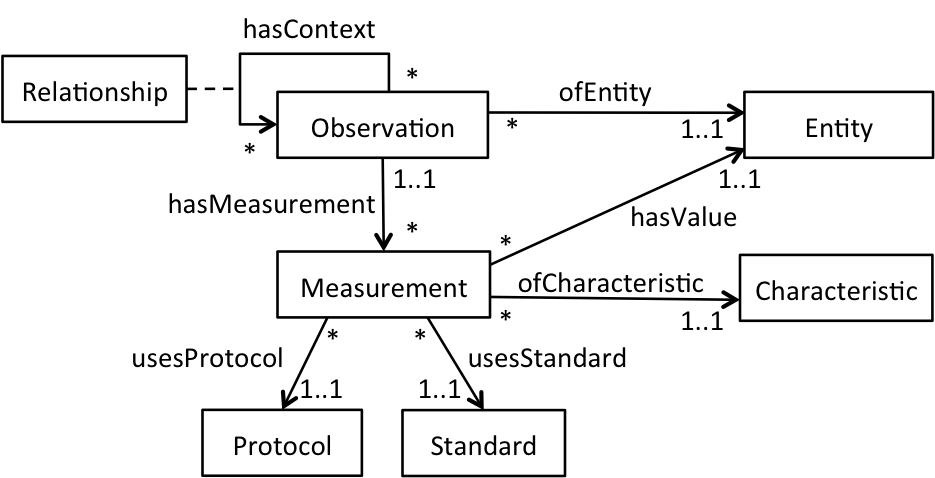
\includegraphics[width=0.5\textwidth]{images/oboe}
  \caption{The main classes and properties of the extensible
    observation ontology (OBOE). While shown using UML, the model is
    defined using OWL-DL.}
  \label{fig:oboe}
\end{figure}

\mypara{Semantic Annotations.} Semantic Annotations describe the
observation model contained in a data object. The Annotation serves as
a template for constructing a fully fleshed OBOE model of the [usually
tabular] data. Less formal descriptions of the data attributes are
often included in traditional metadata formats like EML. while there
is some overlap between these two mechanisms - particularly with
respect to measurement standards or units - semantic concepts applied
to each attribute have the benefit of placing the descriptive burden
on the ontology from which the concepts are drawn. Because the
Annotation represents a potentially subjective perspective on the
data, they are stored independently as XML; the former referencing the
latter.

The Annotation structure largely mirrors the core classes in
OBOE. Observations are composed of Measurements of a specific Entity
and are represented by a collection of Characteristics (usually just
one) collected using a defined Protocol and Standard (i.e. unit).
Tablular data object attributes are mapped to a Measurement such that
a collection of attributes usually pertain to the Entity of a shared
Observation (\figref{fig:kelp-mass-model}). These Observtions can
provide context for other Observations such that the structure of the
observational data model and collection paradigm are formally
represented in the Annotation.


\begin{figure}
\centering
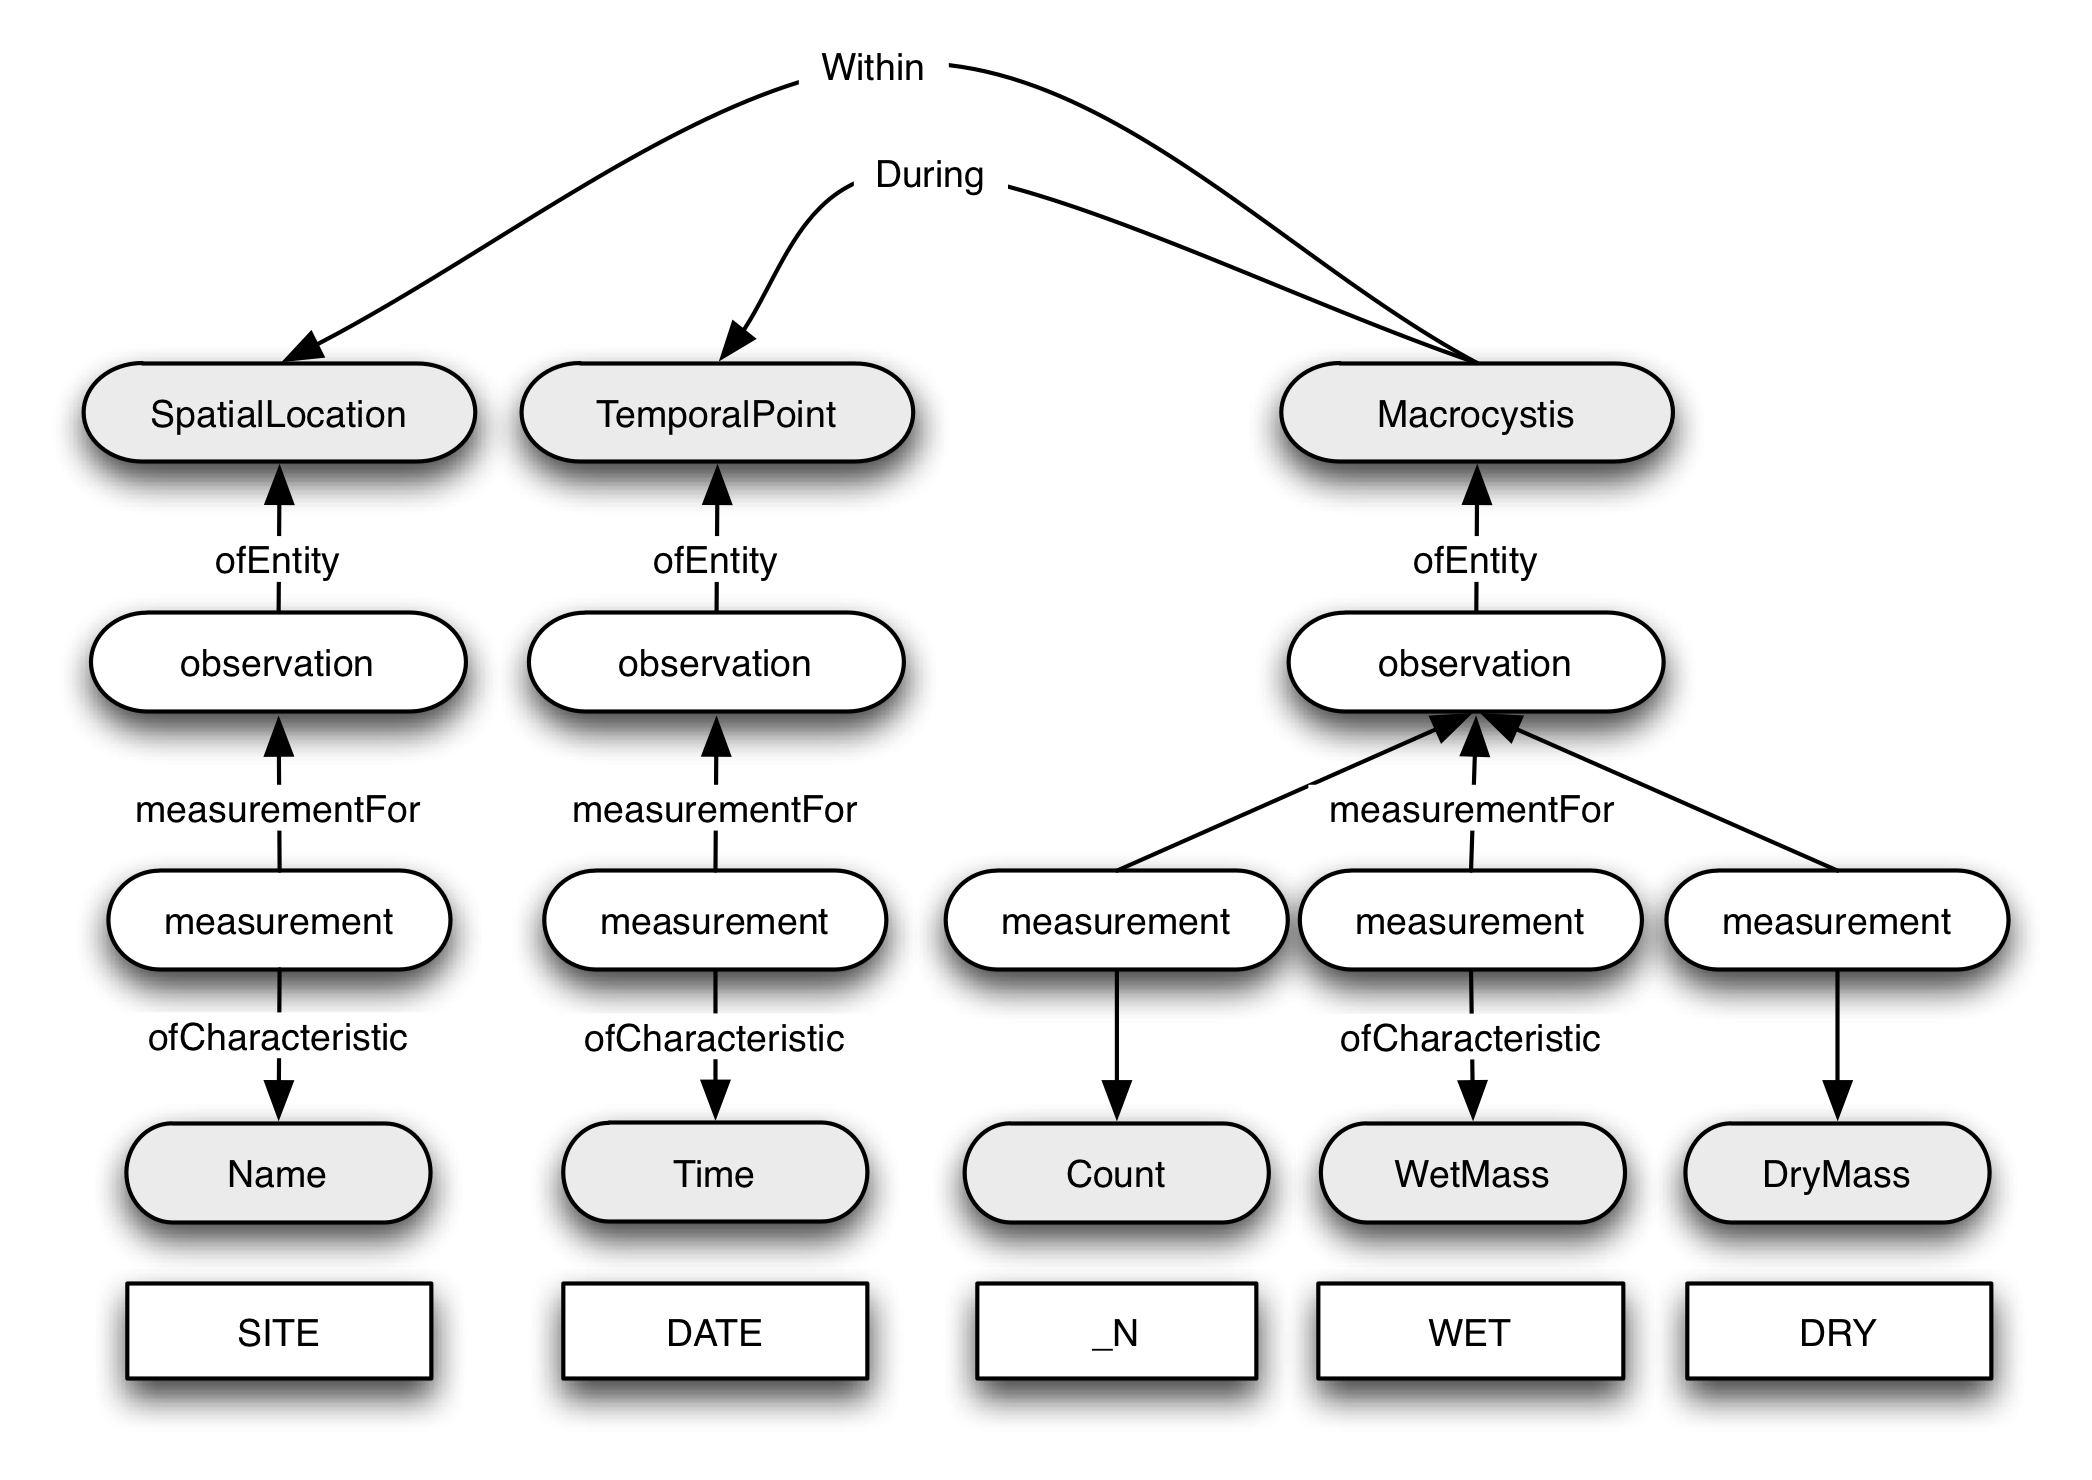
\includegraphics[width=0.5\textwidth]{images/kelp-mass-model.png}
\caption{Partial OBOE Annotation for Kelp sampling data. Shaded nodes represent ontological concepts; rectangular nodes are data table attibutes mapped to OBOE characteristics.}
\label{fig:kelp-mass-model}
\end{figure}


\mypara{The Semantic Mediation API.} The SMS API includes ontology
management features, annotation manipulation capabilities, and simple
concept navigation and visualization widgets. The API is intended to
be a centralized toolkit for use in multiple contexts - be they client
or server - that abstracts the specifics of any single semantic
library. That being said, OWL API primarily underlies the ontology
management interface providing RDF/OWL parsing and serialization as
well as simple class and property exploration. A Pellet reasoner
exposes inferred axioms and relationships that are not explicitly
defined in the source ontologies. Inference is particularly powerful
when utilizing OBOE Measurement 'templates' that express exactly what
(Entity and Characteristic) can be observed and how (Standard and
Protocol).

Annotations are ultimately managed and stored in an opaque local
relational database chosen for scalible persistence and query
performance; the overhead of in-memory Annotation queries having
proven to be prohibitively limiting for large sets of data.

\mypara{The Morpho Editor Plugin.}  The semantic editor plugin for
Morpho provides a front-end to the SMS API and allows metadata editors
to build up semantic Annotations for existing data package
descriptions. The editor focuses on a simplictic fill-in-the-blank
style interface with reusable, searchable, hierachical concept
selection widgets (\figref{fig:morpho-annotation}). The optional
plugin seamlessly integrates with a standard Morpho installation
augmenting the existing features to provide semantic query
capabilities for locating data packages, marking up data packages with
semantic Annotations, and saving Annotations locally or to a shared
repository where they can be discovered and explored by a broader
audience.

\begin{figure*}
\centering
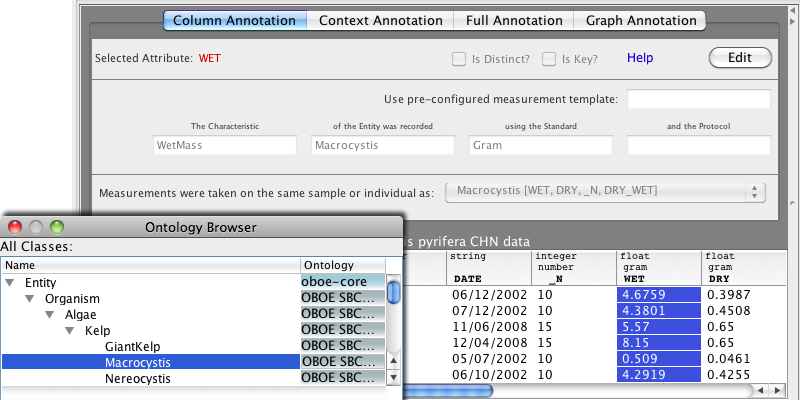
\includegraphics[width=1.0\textwidth]{images/morpho-annotation-widget.png}
\caption{Morpho metadata editor with Semantic plugin. Fill-in-the-blank style editing interface to encourage natural language descriptions. A searchable hierarchical browser is used to select concepts from an ontology.}
\label{fig:morpho-annotation}
\end{figure*}

\mypara{Metacat Query Extensions.}  The semantic plugin for Metacat
augements existing metadata storage and search by allowing Annotations
to be saved and queried alongside the metadata and data that they
annotate. In addition to traditional keyword and spatial search
criteria, the Metacat plugin allows semantic criteria to be included
where they may either increase query recall using term-expansion
(i.e. traversing the class subsumption hierarchy) or refine the
resultset by limiting matches to datasets that contain the specified
observational model (e.g. combinations of OBOE-compatible Entity,
Characteristic, or Protocol concepts). The observational model can be
leveraged further by materializing the Annotation and data artifact
(via the Data Manager Library) into a full OBOE model and inspecting
the observational values themselves.

%%% Local Variables: 
%%% mode: latex
%%% TeX-master: "main"
%%% End: 
